\documentclass{article}
\usepackage{svg}
\usepackage{amsmath}
\usepackage{tipa}
\usepackage{pagecolor,lipsum}
\usepackage{amsfonts}
\usepackage{amssymb}
\usepackage{centernot}
\usepackage{xcolor}
\usepackage{graphicx}
\usepackage{environ}
\NewEnviron{myequation}{%
\begin{equation}
\scalebox{0.8}{$\BODY$}
\end{equation}
}

\begin{document}


\[ \text{Matrix, Lie Group} \]
\[ \text{Rotation matrix} \]
\[
A= \begin{bmatrix}
    \cos(\beta) & -\sin(\beta)\\
    \sin(\beta) & \cos(\beta)
    \end{bmatrix}
\]

\begin{equation}
\begin{aligned}
& A_{\beta=0}= \begin{bmatrix}
    1 & 0\\
    0 & 1 
    \end{bmatrix} \quad
& A_{\beta=\pi/2}= \begin{bmatrix}
    0 & -1\\
    1 & 0 
    \end{bmatrix}\\
& A_{\beta=\pi}= \begin{bmatrix}
    -1 & 0\\
    0 & -1 
    \end{bmatrix}\quad
& A_{\beta=\pi\frac{3}{2}}= \begin{bmatrix}
    0 & 1\\
    -1 & 0 
    \end{bmatrix} \nonumber
\end{aligned}
\end{equation}

\noindent Derive Rotation, Projection and Reflection matrix\\

\noindent Suppose A is the standard matrix for a linear transformation $T: \mathbb{R} \rightarrow \mathbb{R}$
that maps three linear indepedent vectors in $\mathbb{R}$, $x$, $y$, and $z$ as follows:\\
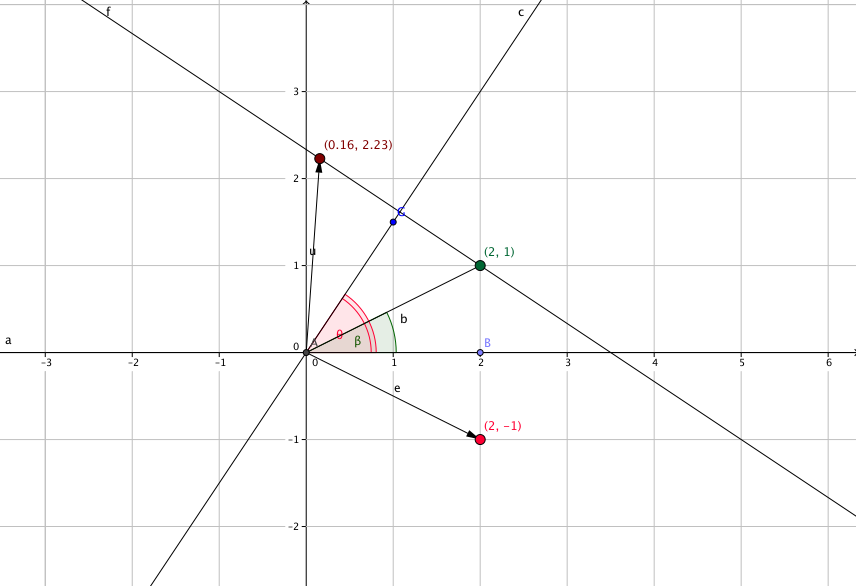
\includegraphics[width=10cm,scale=1]{/Users/cat/myfile/github/image/reflection.png}

\begin{equation}
\begin{aligned}
    & T:x \rightarrow x' \text{ or } & Ax = x'\\
    & T:y \rightarrow y' \text{ or } & Ay = y'\\
    & T:z \rightarrow z' \text{ or } & Az = z'\\
    & \implies A[x, y, z] = [x', y', z']\\
    & \text{let } X = [x, y, z] \text{ and } X' = [x', y', z'] \\
    & \implies AX = X' \\
    & \implies A = X'X^{-1} \\
    & \text{let } X = I \\
    & \implies A = X'
\end{aligned}
\end{equation}
\includegraphics[width=10cm,scale=1]{/Users/cat/myfile/github/image/rotation1.png}

\[ \text{Derive 2 x 2 rotation matrix}\]
\[
 x = \begin{bmatrix}
    1\\
    0 
    \end{bmatrix} \quad \implies \quad
 x'   = \left[
    \begin{array}{c}
      \cos\beta\\
      \sin\beta
      \end{array}
    \right]
\]

\[
 y = \begin{bmatrix}
    0\\
    1 
    \end{bmatrix} \quad \implies \quad
 y'   = \left[
    \begin{array}{c}
      -\sin\beta\\
      \cos\beta
      \end{array}
    \right]
\]
\begin{equation}
\begin{aligned}
& X = \begin{bmatrix}
    1 & 0\\
    0 & 1
\end{bmatrix} \implies
X' = \begin{bmatrix}
    \cos\beta & -\sin\beta\\
    \sin\beta & \cos\beta
\end{bmatrix}\\
& \implies A = 
    \begin{bmatrix}
        \cos\beta & -\sin\beta\\
        \sin\beta & \cos\beta
    \end{bmatrix}
\end{aligned}
\end{equation}

\pagebreak
\[ \text{Derive 2 x 2 projection matrix}\]
\includegraphics[width=10cm,scale=1]{/Users/cat/myfile/github/image/projection.png}

\begin{equation}
\begin{aligned}
    & X' =\left[
    \begin{array}{c}
    l\cos\beta\\
    l\sin\beta
    \end{array}
    \right]
    \quad \text{ and }l = \cos\beta\\
    & \implies X' =\left[
    \begin{array}{c}
    \cos^{2}\beta\\
    \cos\beta\sin\beta
    \end{array}
    \right]\\
    & Y' =\left[
    \begin{array}{c}
    l\cos\beta\\
    l\sin\beta
    \end{array}
    \right]
    \quad \text{ and }l = \sin\beta\\
    & \implies Y' =\left[
    \begin{array}{c}
    \sin\beta \cos\beta\\
    \sin^{2}\beta
    \end{array}
    \right]\\
    & \implies A = 
    \begin{bmatrix}
        \cos^{2}\beta & \sin\beta \cos\beta\\
        \cos\beta \sin\beta & \sin^{2}\beta
    \end{bmatrix}
\end{aligned}
\end{equation}

\pagebreak
\[ \text{Derive 2 x 2 reflection matrix}\]
\includegraphics[width=8cm,scale=1]{/Users/cat/myfile/github/image/reflection1.png}\\
let angle between $l$ and 
$\vec{x} =\left[
    \begin{array}{c}
    1\\
    0
    \end{array}
    \right]
$
is $\beta$\\
so the reflection of $\vec{x}$
is 
$\vec{x'} =\left[
    \begin{array}{c}
    \cos2\beta\\
    \sin2\beta 
    \end{array}
    \right]
$

angle between $l$ and 
$\vec{y} =\left[
    \begin{array}{c}
    0\\
    1 
    \end{array}
    \right]
$
is $\pi/2 - \beta$\\
so the reflection of $\vec{y}$ is  
$\vec{y'} =\left[
    \begin{array}{c}
    \sin2\beta\\
    -\cos2\beta
    \end{array}
    \right]
$\\

\noindent Thereforce the reflection matrix is given by\\
\[
    H = \begin{bmatrix}
        \cos2\beta & \sin2\beta\\
        \sin2\beta & -\cos2\beta
    \end{bmatrix}
\]

\noindent Rotation and reflection matrix form a group\\
\begin{equation}
\begin{aligned}
    R(\beta) = \begin{bmatrix}
        \cos\beta & -\sin\beta\\
        \sin\beta & \cos\beta
    \end{bmatrix}
    H(\alpha) = \begin{bmatrix}
        \cos2\alpha & \sin2\alpha\\
        \sin2\alpha & -\cos2\alpha
    \end{bmatrix} \nonumber
\end{aligned}
\end{equation}
\begin{myequation}
\begin{aligned}
    & R(\beta) \circ R(\alpha) = 
    \begin{bmatrix}
        \cos\beta \cos\alpha - \sin\beta \sin\alpha & -(\cos\beta \sin\alpha + \sin\beta \cos\alpha)\\
        \sin\beta \cos\alpha + \cos\beta \sin\alpha & -\sin\beta \sin\alpha + \cos\beta \cos\alpha 
    \end{bmatrix} & = R(\beta + \alpha)\\
    & R(\beta) \circ H(\alpha) = 
    \begin{bmatrix}
        \cos\beta \cos2\alpha - \sin\beta \sin2\alpha & \cos\beta \sin2\alpha + \sin\beta \cos2\alpha \\
        \sin\beta \cos2\alpha + \cos\beta \sin2\alpha & \cos\beta \cos2\alpha -\sin\beta \sin2\alpha  
    \end{bmatrix} & = H(\alpha + \frac{\beta}{2})\\
    & H(\alpha) \circ R(\beta) = 
    \begin{bmatrix}
        \cos2\alpha\cos\beta + \sin2\alpha \sin\beta & \cos 2\alpha \sin\beta + \sin2\alpha\cos\beta \\
        \sin2\alpha \cos\beta - \cos2\alpha \sin2\beta & -\cos2\alpha \sin\beta - \cos2\alpha \cos\beta
    \end{bmatrix} & = H(\alpha - \frac{\beta}{2})\\
    & H(\beta) \circ H(\alpha) = 
    \begin{bmatrix}
        \cos2\beta \cos2\alpha + \sin2\beta \sin2\alpha & \cos2\beta \sin2\alpha - \sin2\beta \cos2\alpha \\
        \cos2\beta \sin2\alpha - \cos2\beta \sin2\alpha & \sin2\beta \sin2\alpha + \cos2\beta \cos2\alpha 
    \end{bmatrix} & = R(2(\alpha - \beta)) \nonumber
\end{aligned}
\end{myequation}

$\langle R(\beta) , H(\alpha) \rangle $ generates a group\\

\noindent 
The determinant of the rotation $\det(R) = \cos^{2}\beta + \sin^{2}\beta = 1$\\
The determinant of the reflection $\det(H) = -(\cos^{2}2\alpha+ \sin^{2}2\alpha)= -1$\\

\noindent Exponential map
$exp(A) = \sum_{k=0}^{n} \frac{A^{k}}{k!}$\\
If A is n by n matrix, then prove the series is converage\\

\begin{equation}
\begin{aligned}
    \exp(A)  & = \sum_{k=0}^{n} \frac{A^{k}}{k!} \\
    \sin(A)  & = \sum_{k=0}^{n} (-1)^{k}\frac{A^{2k}}{2k!} \\
    \cos(A)  & = \sum_{k=0}^{n} (-1)^{k}\frac{A^{2k+1}}{(2k+1)!} \\
    \cosh(A) & = \sum_{k=0}^{n} \frac{A^{2k}}{(2k)!} \\
    \sinh(A) & = \sum_{k=0}^{n} \frac{A^{2k+1}}{(2k+1)!}  \nonumber
\end{aligned}
\end{equation}

\noindent
Let $ A = 
    \begin{bmatrix}
    0 & -\beta \\
    \beta & 0 
    \end{bmatrix}
$\\
$
    \exp(A) = 
        \begin{bmatrix}
        1 & 0 \\
        0 & 1 
        \end{bmatrix}
        +
        \begin{bmatrix}
        0 & -\beta \\
        \beta & 0 
        \end{bmatrix}
        +
        \frac{1}{2!}
        \begin{bmatrix}
        -\beta^{2} & 0 \\
        0 & \beta^{2} 
        \end{bmatrix}
        +
        \frac{1}{3!}
        \begin{bmatrix}
        0 & \beta^{3} \\
        -\beta^{3} & 0 
        \end{bmatrix}
        +
        \frac{1}{4!}
        \begin{bmatrix}
        \beta^{4} & 0 \\
         0 & \beta^{4} 
        \end{bmatrix}
        +
        \frac{1}{5!}
        \begin{bmatrix}
        0 & -\beta^{5}\\
        \beta^{5} & 0 
        \end{bmatrix}
$\\

$
    \exp(A) = 
        \begin{bmatrix}
        1 + \frac{1}{2!}(-\beta^{2}) + \frac{1}{4!}\beta^{4} + ... & -\beta + \frac{1}{3!}\beta^{3} + ...\\
        \beta + \frac{1}{3!}-\beta^{3} + ... & 1 + \frac{1}{2!}\beta^{2} + \frac{1}{4!}\beta^{4} + ...
        \end{bmatrix}
        = 
        \begin{bmatrix}
        \sin(\beta) & -\cos(\beta)\\
        \cos(\beta) & \sin(\beta)
        \end{bmatrix}
$

            \begin{equation}
            \begin{aligned}
                M_{z}(\theta) & =\begin{bmatrix}
                        \cos\theta & -\sin\theta & 0\\
                        \sin\theta & \cos\theta & 0\\   
                        0      &   0    & 1  
                    \end{bmatrix}  & = \left. \frac{d M_z}{d \theta} \right\rvert_{\theta=0} 
            \end{aligned}
            \end{equation}

\end{document}

